\subsection{Mosaicity}
\label{sec:mosaicity}
A two-dimensional powder is already random in in-plane azimuth. Mosaicity adds a distribution of crystallite tilts about the mean film normal. Its role is visible in the measured detector image in Fig.~\ref{fig:hk0_low_l_star}, where it explains features that are otherwise incompatible with a single incident vector and one perfectly aligned crystallite.

Figure~\ref{fig:hk0_low_l_star} shows the $r=0$ region of a Bi$_2$Se$_3$ image collected at the nominal incident angle $\theta_i=5^\circ$. That incident condition places the Ewald intersection near the $003$ condition. Surprisingly, intensity is also visible near the $006$ location, at approximately twice the radial $2\theta$ coordinate of $003$. The $003$ feature is also strongly anisotropic: its long extension follows the radial $2\theta$ direction, whereas its transverse width follows the outgoing-ray azimuth $\phi$.

For the $003$ peak, the transverse $\phi$ width is primarily due to mosaicity, while the radial spread is better explained by wavelength dispersion. As discussed below, the unexpected $006$ intensity motivates testing a broad component in the mosaic distribution. The bright feature near $L=0$ is specular reflectivity, discussed separately in Sec.~\ref{sec:reflectivity}.


\begin{figure}[H]
  \centering
  \textbf{Radial and transverse structure of the Bi$_2$Se$_3$ $r=0$ region}
  \begin{minipage}{0.92\linewidth}
    \centering
    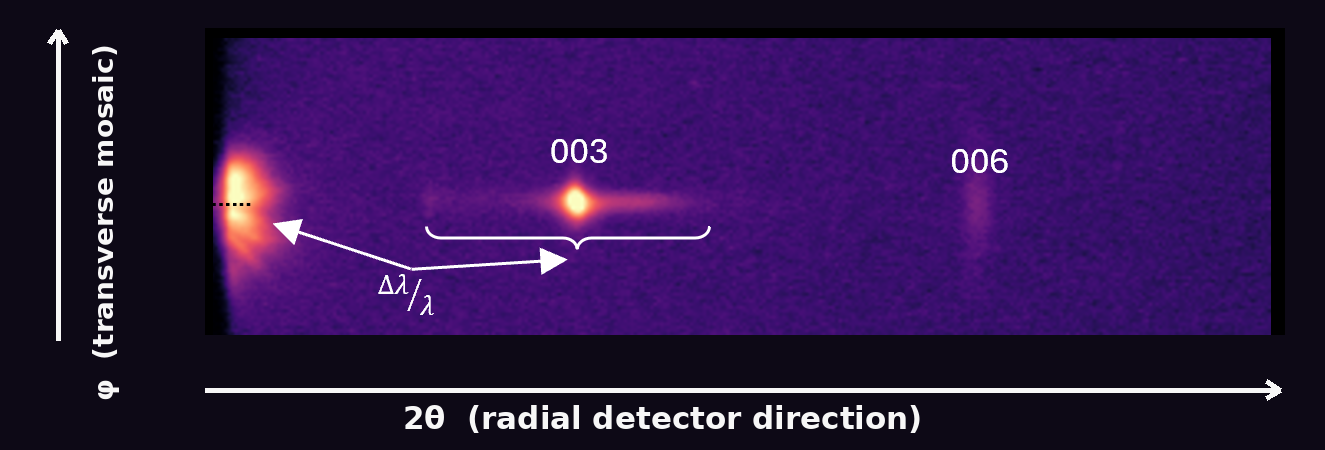
\includegraphics[width=\linewidth]{figures/results_ordered/00L_region_wavelength_mosaic_axes.png}
  \end{minipage}
  \caption{Measured $r=0$ detector region from the $5^\circ$ Bi$_2$Se$_3$ image. The nominal incident condition lies near $003$, while intensity is also observed near the $006$ location at approximately twice its radial $2\theta$ coordinate. The $003$ feature has a long radial extension along $2\theta$, whereas its transverse $\phi$ width is the cleaner constraint on crystallite tilt. The bright near-origin feature is near-critical specular reflectivity discussed in Sec.~\ref{sec:reflectivity}.}
  \label{fig:hk0_low_l_star}
\end{figure}

As shown below, off-specular rod-family arcs and the transverse $\phi$ width of off-condition $r=0$ intensity probe different parts of the same orientation distribution. Strong off-specular arcs mainly constrain crystallites whose normals are close to the mean film normal. Weak $r=0$ intensity farther from the specular direction is more sensitive to the small population at larger tilt.

To apply the crystallite mosaic tilt, we rotate each point on the powder cylinder through $\alpha$ about its local in-plane tilt axis,
\begin{equation}
  \mathbf Q_{hk}(\alpha,\beta,L)
  =\mathbf R_{\widehat{\mathbf b}_t(\beta)}(\alpha)
   \mathbf Q^{\mathrm{cyl}}_{hk}(\beta,L),
  \label{eq:mosaic_orientation_map}
\end{equation}
where $\alpha$ is the crystallite-tilt magnitude and $\beta$ is the cylinder azimuth. The local unit tilt axis is
\[
  \widehat{\mathbf b}_t(\beta)
  =\mathbf C\,\mathbf R_{\widehat{\mathbf c}^{\,*}}(\beta)
   \widehat{\mathbf b}_t^{\,0},
\]
where $\widehat{\mathbf b}_t^{\,0}$ is the reference in-plane unit axis. Thus, the tilt axis rotates with the cylinder azimuth $\beta$. At $\alpha=0$, Eq.~\eqref{eq:mosaic_orientation_map} reduces to the powder cylinder in Eq.~\eqref{eq:powder_cylinder}.

The data were reproduced by a distribution with long tails,
\begin{equation}
  \omega_{\mathrm w}(\alpha;p_{\mathrm{tail}},\Gamma,\sigma)
  =p_{\mathrm{tail}}L_{\mathrm w}(\alpha;\Gamma)
  +(1-p_{\mathrm{tail}})G_{\mathrm w}(\alpha;\sigma),
  \qquad 0\le p_{\mathrm{tail}}\le1,
  \label{eq:mosaic_two_component_maintext}
\end{equation}
with the normalized orientation density
\begin{equation}
  p_m(\alpha,\beta)=\frac{\omega_{\mathrm w}(\alpha;p_{\mathrm{tail}},\Gamma,\sigma)}{2\pi},
  \qquad
  \int_0^\pi\!\int_0^{2\pi}p_m(\alpha,\beta)\,d\beta\,d\alpha=1.
  \label{eq:mosaic_orientation_density}
\end{equation}
Here $G_{\mathrm w}$ is the Gaussian-like narrow core, $L_{\mathrm w}$ is the Lorentzian-like broad component, and $p_{\mathrm{tail}}$ is its weight. The two components share one center but have independent widths. The Lorentzian-like form is not a claim that the physical distribution is uniquely Lorentzian.

Figure~\ref{fig:mosaic_combo} explains the geometric sensitivity to a broad component. For $r\neq0$, the strong detector arcs sample the orientation range near the nominal reciprocal vector. The transverse extent of off-condition $r=0$ intensity probes larger tilts. Establishing that the broad component is necessary still requires a same-fit no-tail comparison and a fairly re-optimized Gaussian-only model, with residuals and uncertainty across the measured incident angles.

\begin{figure}[htbp]
  \centering
  \captionsetup[subfigure]{list=false,labelsep=none}

  \begin{subfigure}[t]{0.48\linewidth}
    \centering
    \paneltagged{(a)}{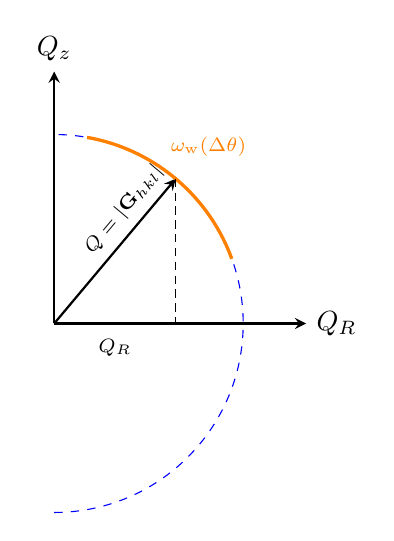
\begin{tikzpicture}[scale=2,>=stealth]
  \def\R{1.2}        % Bragg-sphere radius
  \def\Raxis{1.6}    % axis length
  \def\angleMid{50}  % midpoint angle of mosaic arc (degrees)

  % Folded Bragg locus in the radial coordinate Q_R >= 0
  \draw[dashed,blue] (0,-\R) arc (-90:90:\R);

  % reciprocal-space axes
  \draw[->,thick] (0,0) -- (0,\Raxis) node[above] {$Q_z$};
  \draw[->,thick] (0,0) -- (\Raxis,0) node[right] {$Q_R$};

  % radius vector at midpoint of mosaic arc, label closer to tip
  \coordinate (Gvec) at ({\R*cos(\angleMid)},{\R*sin(\angleMid)});
  \draw[thick,->] (0,0) -- (Gvec)
       node[pos=0.7, above, sloped] {\scriptsize $Q=|\mathbf G_{hkl}|$};

  % mosaic arc on the Bragg sphere, labeled with omega(theta)
  \draw[very thick,orange]
    ({\R*cos(20)},{\R*sin(20)}) arc (20:80:\R)
    node[pos=0.6, above right] {\scriptsize $\omega_{\mathrm w}(\Delta\theta)$};

  % projection onto the radial reciprocal-space axis
  \coordinate (Gr) at ({\R*cos(\angleMid)},0);
  \draw[densely dashed] (Gvec) -- (Gr);
  \node[below, yshift = -2pt] at ({0.5*\R*cos(\angleMid)},0) {\scriptsize $Q_R$};

\end{tikzpicture}
}
    \phantomcaption
    \label{fig:mosaic_combo:schem_inplane}
  \end{subfigure}\hfill
  \begin{subfigure}[t]{0.48\linewidth}
    \centering
    \paneltagged{(b)}{\begin{tikzpicture}[scale=2,>=stealth]
  \def\R{1.2}
  \def\Raxis{1.6}
  \def\angleMid{90}

  % Folded Bragg locus in the radial coordinate Q_R >= 0
  \draw[dashed,blue] (0,-\R) arc (-90:90:\R);

  % Reciprocal-space axes
  \draw[->,thick] (0,0) -- (0,\Raxis) node[above] {$Q_z$};
  \draw[->,thick] (0,0) -- (\Raxis,0) node[right] {$Q_R$};

  % Specular reciprocal vector
  \coordinate (Gvec) at ({\R*cos(\angleMid)},{\R*sin(\angleMid)});
  \draw[thick,->] (0,0) -- (Gvec)
       node[pos=0.75, right] {\scriptsize $Q=|\mathbf G_{00l}|$};

  % Narrow core near the axis and broad component at larger tilt
  \draw[very thick,oiPurple]
    ({\R*cos(80)},{\R*sin(80)}) arc (80:90:\R)
    node[pos=0.45, above right, text=oiPurple] {\scriptsize narrow core};
  \draw[very thick,oiOrange,dashed]
    ({\R*cos(55)},{\R*sin(55)}) arc (55:80:\R)
    node[pos=0.45, right, text=oiOrange] {\scriptsize broad component};
\end{tikzpicture}
}
    \phantomcaption
    \label{fig:mosaic_combo:schem_specular}
  \end{subfigure}

  \vspace{0.6em}

  \begin{subfigure}[t]{0.48\linewidth}
    \centering
    \paneltagged{(c)}{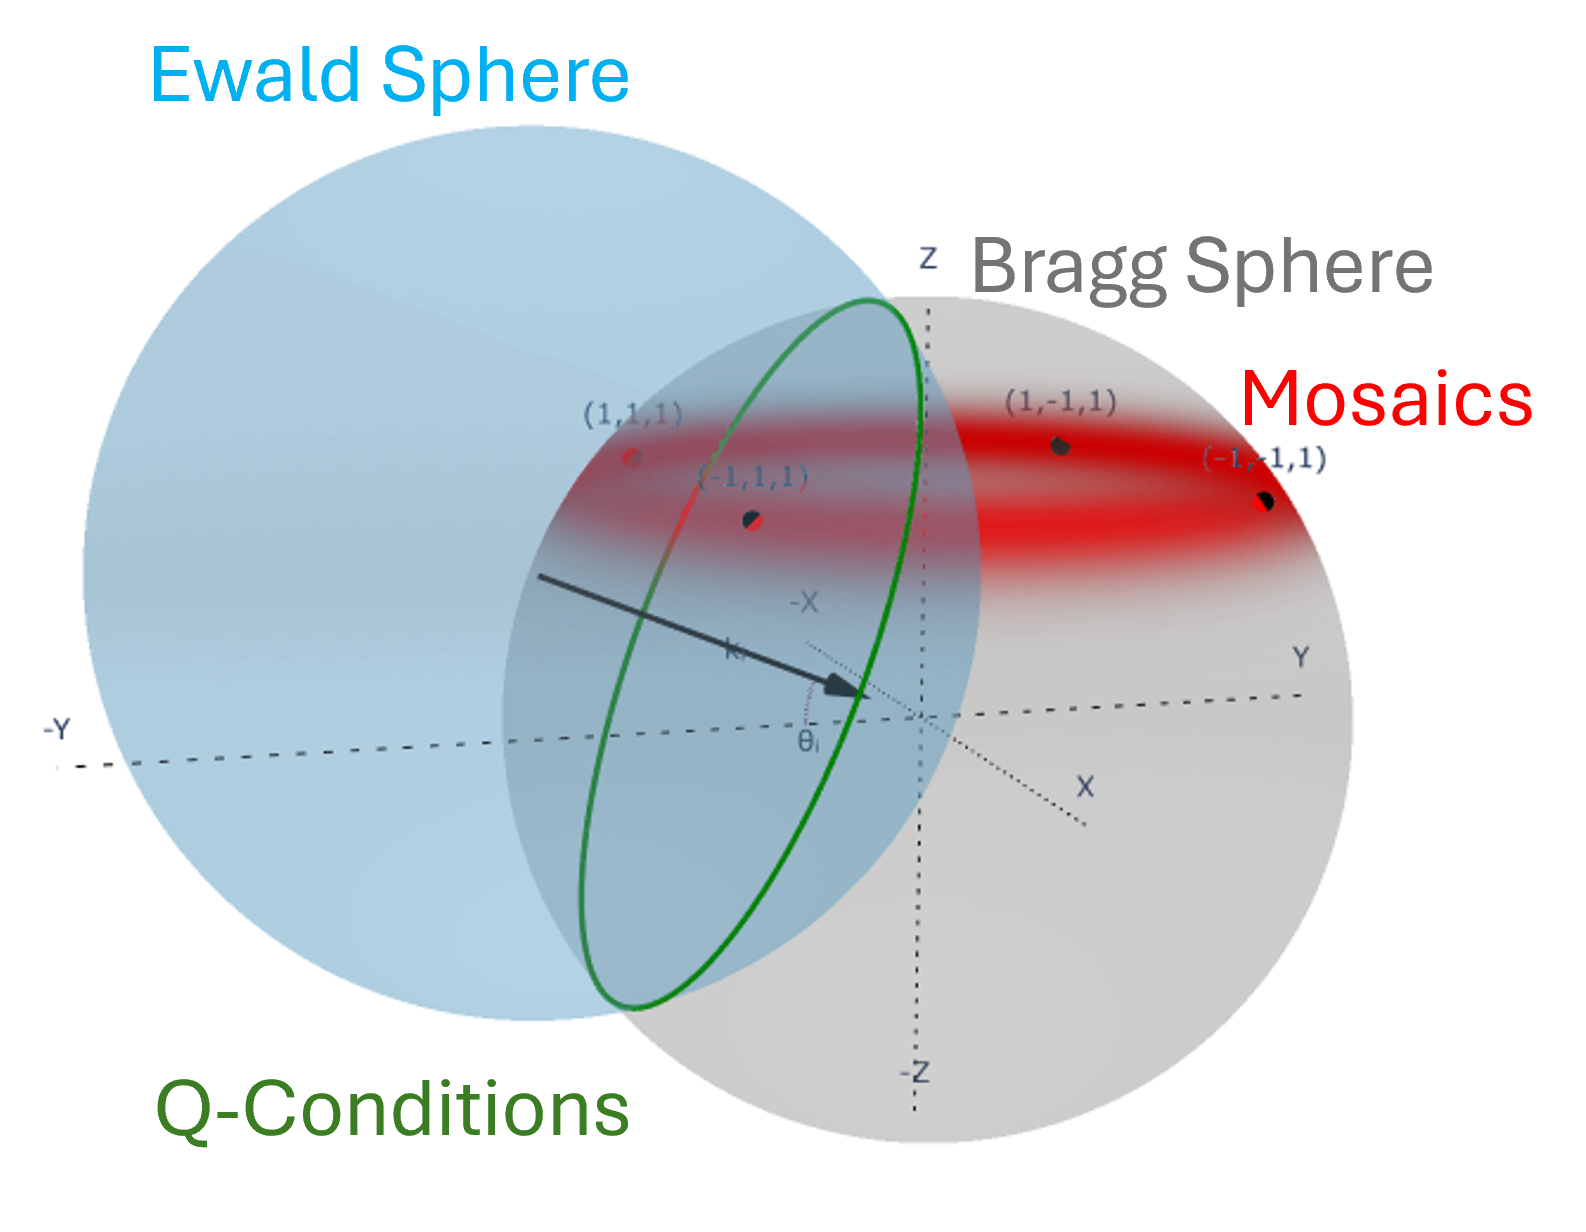
\includegraphics[width=\linewidth]{figures/mosaic/inplane_detector_band.png}}
    \phantomcaption
    \label{fig:mosaic_combo:img_inplane}
  \end{subfigure}\hfill
  \begin{subfigure}[t]{0.48\linewidth}
    \centering
    \paneltagged{(d)}{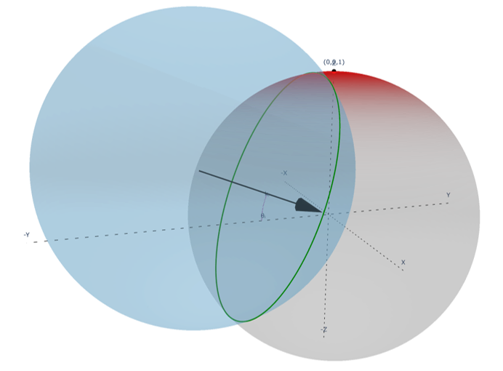
\includegraphics[width=\linewidth]{figures/mosaic/specular_detector_cap.png}}
    \phantomcaption
    \label{fig:mosaic_combo:img_specular}
  \end{subfigure}

  \caption{Geometric sensitivity to the narrow and broad crystallite-tilt components. (a) For $r\neq0$, the reciprocal vector has radial and film-normal components $Q_R$ and $Q_z$. The purple segment identifies the narrow core that predominantly controls the strong off-specular arc width, while the dashed orange extension identifies the broad, low-probability component. (b) For $r=0$, the same orientation distribution begins on the film-normal axis. Intensity displaced in the transverse $\phi$ direction samples larger crystallite tilts and is therefore more sensitive to the broad component. This transverse mosaic effect is distinct from the radial $2\theta$ streak through $003$, which is assigned primarily to wavelength dispersion in Fig.~\ref{fig:hk0_low_l_star}. Opposite tilts fold onto the same $Q_R\ge0$ locus. (c,d) Three-dimensional views place the corresponding orientation distributions relative to the Ewald-sphere intersection. The schematic illustrates sensitivity and does not replace a controlled mosaic-component comparison.}
  \label{fig:mosaic_combo}
\end{figure}
